\section{Specifications}
\label{sec:specs}
\newcounter{SpecID}

\subsection{Arena}
\refstepcounter{SpecID}
\label{spec:arena}

\begin{enumerate}
  \item The arena floor is an \SI{8}{m} UPDATE $\times$ \SI{8.1}{m} rectangle. The
        tolerance of these two dimensions is $\pm$ \SI{250}{mm}.
  \item The floor of the arena is carpeted.
  \item The layout of the arena is given in Figure~\ref{fig:arena}. This
        figure is to scale.
  \item The outer walls of the arena are at least \SI{600}{mm} high, and the
        interior surface is white plastic-coated hardboard.
  \item The starting location of the robots is given in Figure~\ref{fig:arena}.
        Teams are allowed to place their robot anywhere such that the entire
        robot is within \SI{1}{m} of the starting point, which will be
        indicated on the floor of the arena.
  \item The scoring zones are given in Figure~\ref{fig:arena} and are marked out
        on the arena floor.
\end{enumerate}

\begin{figure}
  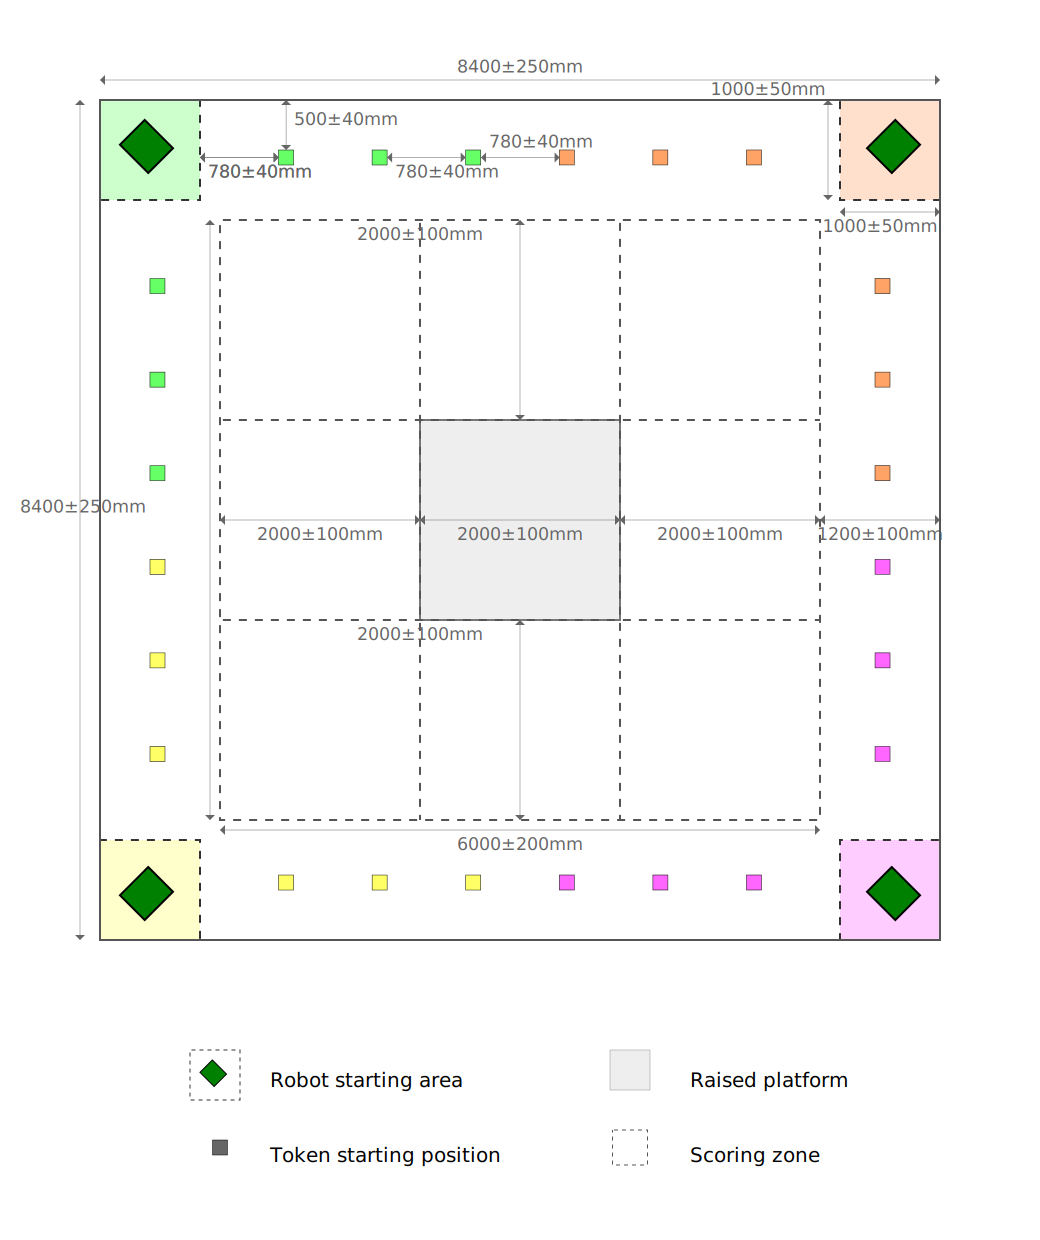
\includegraphics[scale=0.58]{fig-arena.pdf}
  \caption{Layout zones and cans in the arena.}
  \label{fig:arena}
\end{figure}

\subsection{Markers}
\refstepcounter{SpecID}
\label{spec:markers}

The arena, and Apples, are labelled with fiducial markers. Each
marker number is associated with a particular feature in the arena,
and also has an associated size.  The marker numbers and sizes are
as follows:

\begin{center}
\begin{tabular}{lcc}
  \toprule
  \textbf{Item} & \textbf{Marker Number} & \textbf{Marker Size (\si{mm})} \\
  \midrule
  Arena boundary  &     0 -- 27   &   250 \\
  Golden Apples   &     28 -- 31  &   80  \\
  Other Apples (including Red and Rotten Apples) & 32 -- 40 & 80 \\
  \bottomrule
\end{tabular}
\end{center}

\subsection{Apples}
\refstepcounter{SpecID}
\label{spec:apples}

\begin{enumerate}
  \item 'Apples' are cubes of side length \SI{100}{mm}($\pm$\SI{10}{mm}).
  \item They are made of cardboard and have markers on them as detailed in \ref{spec:markers}
  \item Aditionally, each cube has conductive tape on all edges and has internal
        circuitry equivalent to a capacitor in parallel with a resistor of large value
        on the order of $\approx\SI{1}{M\ohm}$.
  \item The capacitance value varies between cubes as follows:
  \begin{center}
      \begin{tabular}{lcc}
            \toprule
            \textbf{Apple Type}     &     \textbf{Capacitance (\si{nF})}    \\
            \midrule
            Red Apple               &     a UPDATE       \\
            Golden Apple            &     b UPDATE       \\
            Rotten Apple            &     c UPDATE       \\
            \bottomrule
      \end{tabular}
  \end{center}

\end{enumerate}

\subsection{Scoring zone}
\refstepcounter{SpecID}
\label{spec:scoringZone}

\begin{enumerate}
      \item Each robot will have a scoring zone as specified in \ref{fig:arena}.
      \item Robots score points by putting Apples in their respective scoring zone.
      \item In each socing zone is a 'Market stall' with the dimensions in TODO ref{}
\end{enumerate}
